%-----------------------------------LICENSE------------------------------------%
%   This file is part of Mathematics-and-Physics.                              %
%                                                                              %
%   Mathematics-and-Physics is free software: you can redistribute it and/or   %
%   modify it under the terms of the GNU General Public License as             %
%   published by the Free Software Foundation, either version 3 of the         %
%   License, or (at your option) any later version.                            %
%                                                                              %
%   Mathematics-and-Physics is distributed in the hope that it will be useful, %
%   but WITHOUT ANY WARRANTY; without even the implied warranty of             %
%   MERCHANTABILITY or FITNESS FOR A PARTICULAR PURPOSE.  See the              %
%   GNU General Public License for more details.                               %
%                                                                              %
%   You should have received a copy of the GNU General Public License along    %
%   with Mathematics-and-Physics.  If not, see <https://www.gnu.org/licenses/>.%
%------------------------------------------------------------------------------%
%       Author: Ryan Maguire                                                   %
%       Date:   2023/10/14                                                     %
%------------------------------------------------------------------------------%
\documentclass{article}
\usepackage[margin=1in]{geometry}
\usepackage{amssymb}
\usepackage{amsthm}
\usepackage{amsmath}
\usepackage[font=scriptsize,
            labelformat=simple,
            labelsep=colon]{subcaption} % Subfigure captions.
\usepackage[font={scriptsize},
            hypcap=true,
            labelsep=colon]{caption}    % Figure captions.
\usepackage{graphics}
\usepackage{hyperref}

\hypersetup{colorlinks=true, linkcolor=blue}

\theoremstyle{plain}
\newtheorem{theorem}{Theorem}
\newtheorem{conjecture}{Conjecture}
\newtheorem{question}{Question}

\title{Research Statement}
\author{Ryan Maguire}
\date{\today}

\begin{document}
    \maketitle
    \section{Introduction}
        My research interests lie in knot theory, topology, and Lorentz
        geometry, with a particular captivation in numerical methods and the
        design of algorithms. Knot theory is a challenging field when it comes
        to numerical analysis, many of the procedures have aweful complexities.
        For a simple example, it has been known since the 1920s
        (Reidemeister \cite{Reidemeister1927}, Alexander and Briggs
        \cite{AlexanderBriggs1926}) that two knot diagrams are isomorphic as
        knots if and only if there is a finite sequence of Reidemeister moves
        between them. In \cite{HassLagarias2001} Hass and Lagarias found an
        explicit upper bound for the number of moves required to convert an
        unknot with $n$ crossings to its usual zero crossing diagram. The
        bound is $2^{cn}$ where $c$ is the constant $10^{11}$.%
        \footnote{%
            The authors remarked that this can be improved.
            If we input $n=1$ we get an upper bound of
            $2.5\times{10}^{30,102,999,566}$ Reidemeister moves,
            when the minimum required is 1!
        }
        Heinrich and Kauffman found a factorial expression that only grows
        larger than this exponential formula for knots with more than
        $10^{10^{10}}$ crossings \cite{HenrichKauffman2010Unknotting}, and
        more recently a polynomial bound of
        $(236n)^{11}$ was found by Lackenby \cite{Lackenby2015Unknotting}.
        \par\hfill\par
        A simple algorithm for detecting if any knot diagram corresponds to the
        unknot can be made using these bounds. Loop through all possible
        combinations of Reidemeister moves of length $(236n)^{11}$ for your
        initial $n$ crossing knot diagram and if you never
        find the standard diagram for the unknot you know you've got something
        different. In practice the universe will reset itself before your
        algorithm terminates when implemented on real hardware.%
        \footnote{%
            There are around $3^{(236n)^{11}}$ combinations of Reidemeister
            moves. Inputting $n=2$ yields roughly $10^{10^{29}}$ combinations
            to check. The age of the universe is about $10^{18}$ seconds.
        }
        Other methods must be devised to make this problem approachable.
        In 2011 Kronheimer and Mrowka proved that Khovanov homology detects the
        unknot \cite{KronheimerMrowka2011KhovanovUnknot} and Bar-Natan's 2006
        paper provides an efficient means of computing this
        \cite{BarNatan2006FASTKH}, running (experimentally) like
        $O(2^{\sqrt{n}})$ where $n$ is the number of crossings. Most recently
        Lackenby developed an algorithm that runs in
        $O(2^{\log(n)^{3}})$, quasi-polynomial time
        \cite{LackenBy2021QuasiPolyUnknotting}. The complexity of this problem
        has been well studied. In 2014 Kuperberg proved (assuming the generalized
        Riemann hypothesis is true) that knottedness is both \texttt{NP} and
        \texttt{co-NP} \cite{Kuperberg2014KnottednessNP}. Lackenby soon after
        proved the same result without the assumption of the generalized
        Riemann hypothesis \cite{Lackenby2021UnknotNP}.
        \par\hfill\par
        It is hoped the above paragraphs have convinced one that even simple
        problems (recognizing the unknot) in knot theory are challening,
        both theoretically (performing the mathematics and designing the
        algorithms), and practically (implementing the algorithms
        in a programming language).
        My personal contributions lie in the implementation of knot algorithms
        for the tabulation of knot invariants. For a simple example,
        consider the Jones polynomial. Given an $n$ crossing knot $K$
        with crossings ordered between $0$ and $n-1$ we can define the
        Kauffman bracket via:
        \begin{equation}
            \langle{K}\rangle(q)
            =\sum_{k=0}^{2^{n}-1}(-q)^{w(k)}(q+q^{-1})^{c(k)}
        \end{equation}
        Where $w(k)$ is the Hamming weight of $k$, the number of 1's that occur
        in the binary expansion of $k$, and $c(k)$ is the
        \textit{circle counting function}. That is, given a number
        $0\leq{k}\leq{2}^{n}-1$ we write $k$ in binary. If the $m^{th}$ bit is
        zero we performed a zero-smoothing at the $m^{th}$ crossing of $K$,
        otherwise we perform a one-smoothing. Every bit of $k$ tells us how to
        smooth all of the crossings (See Fig.~\ref{fig:cube_of_resolutions}).
        \begin{figure}
            \centering
            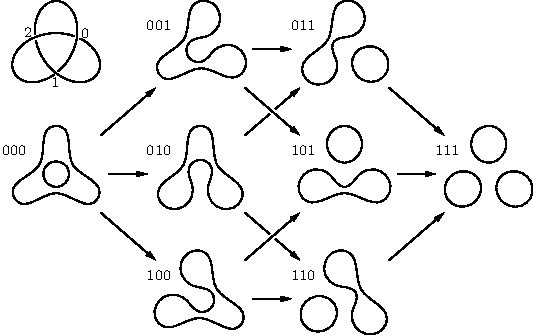
\includegraphics{trefoil_knot_cube_of_resolutions.pdf}
            \caption{Cube of Resolutions for the Trefoil}
            \label{fig:cube_of_resolutions}
        \end{figure}
        The result is the disjoint union of
        cycles in the plane. $c(k)$ counts the number of cycles corresponding
        to $k$. The Jones polynomial $J(K)$ is a normalization of
        $\langle{K}\rangle$ in terms of the writhe of $K$. Computing the writhe
        is linear in time, and the normalization step runs in constant time
        (shifting the minimum degree of the polynomial). This can be ignored for
        the purposes of algorithm design. The na\"{i}ve brute-force formula
        above yields an algorithm that is $O(2^{n})$, assuming that
        polynomial multiplication and addition run in constant time.
        Many improvements have been made over the years, and several
        algorithms exist (\cite{Thistlethwaite1987SpanningTreeJones},
        \cite{Zulli1995MatrixForJonesPolynomial},
        \cite{ElMisieryElHorbatyJonesAlgorithm},
        \cite{Gousbet2001JonesAlgorithm},
        \cite{MustafaLevitt2018JonesAlgorithm}), and even quantum algorithms
        (See \cite{JonesQuantumAlgorithm} and \cite{Lomonaco2008AQM}).
        Implementations have been made
        and optimized (\cite{sage}, \cite{regina},
        \cite{SnapPy}, \cite{libtmpl})
        allowing for the tabulation of the Jones polynomial of
        all prime knots with up to 19 crossings
        \cite{JonesData}. Similar efforts exist for the HOMFLY-PT polynomial
        (\cite{Gousbet1999HOMFLYAlgorithm},
        \cite{Burton2018HOMFLFixedParameter},
        \cite{Burton2012ComputationalTW}),
        a bivariate Laurent polynomial that generalizes the Jones polynomial,
        and a database has been created (\cite{HOMFLYData}). I have parallelized
        some of the scripts, and this table can be created in a few hours.%
        \footnote{%
            The table consists of over 352 million knot polynomials. Not bad
            for a sub-exponential algorithm.
        }
        \par\hfill\par
        The Khovanov polynomial is defined from Khovanov homology by throwing
        away the torsion components, summing over the dimension of the
        homogeneous components
        $KH_{n}^{m}(K)$:
        \begin{equation}
            Kh(K)(q,\,t)=\sum_{m,\,n}
                q^{n}t^{m}\textrm{dim}\big(KH_{n}^{m}(K)\big)
        \end{equation}
        This contains the Jones polynomial, $J(K)(q)=Kh(q,\,-1)$. Efforts to
        tabulate the Khovanov polynomial have proven difficult, but all prime
        knots up to 17 crossings have been completed \cite{KhovanovData}.%
        \footnote{%
            Attempts to parallelize these procedures is underway to get to
            19 crossings in a reasonable amount of time.
        }
        \par\hfill\par
        I have used these tables and programs to experiment with conjectures in
        knot theory and contact topology. A contact structure on a
        $2n+1$ dimensional manifold $M$ is a distribution of hyperplanes in the
        tangent bundle of $M$ satisfying a \textit{maximal non-integrability}
        condition. Locally this means it is given by a 1-form $\alpha$ such
        that $\alpha\land(\textrm{d}\,\alpha)^{n}\ne{0}$. The standard contact
        structure on $\mathbb{R}^{3}$ can be given globally by
        $\alpha=\textrm{d}z-y\textrm{d}x$, the hyperplane at $(x,\,y,\,z)$
        being spanned by the vectors $\partial_{x}+y\partial_{z}$ and
        $\partial_{y}$ (See Fig.~\ref{fig:darboux_form}). The maximal
        non-integrability conditions means that there is no surface that,
        neither locally nor infinitesimally, has its tangent planes given by
        the hyperplane distribution.
        \begin{figure}
            \centering
            \resizebox{0.8\textwidth}{!}{%
                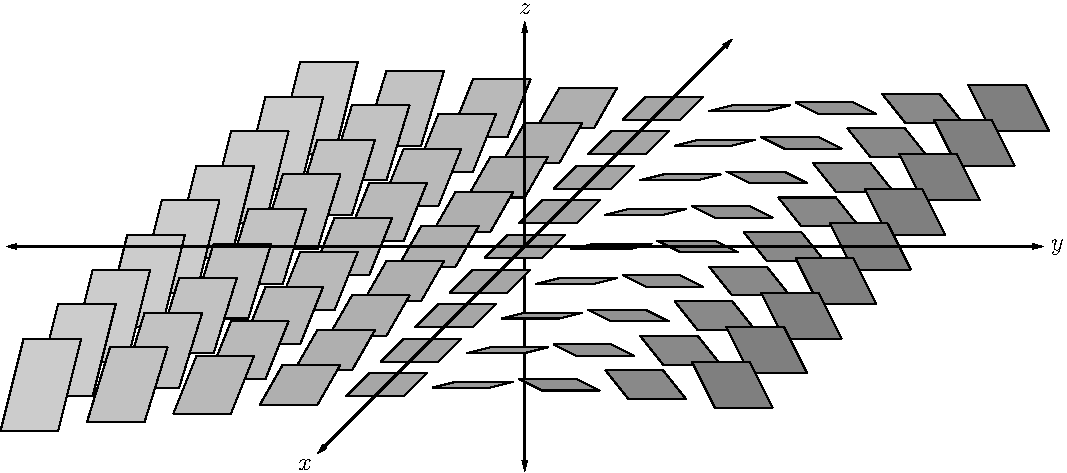
\includegraphics{darboux_form_001.pdf}
            }
            \caption{Standard Contact Structure for $\mathbb{R}^{3}$}
            \label{fig:darboux_form}
        \end{figure}
        It is, however, possible for curves to be everywhere tangent to the
        contact structure. These are called \textit{Legendrian submanifolds}.
        Legendrian knots are smooth embeddings of $\mathbb{S}^{1}$ into
        $\mathbb{R}^{3}$ that are also Legendrian submanifolds. Legendrian
        knot theory studies Legendrian knots up to \textit{Legendrian isotopy},
        a smooth family $H_{t}$, $t\in[0,\,1]$, of Legendrian knots. It is
        possible for two embeddings of $\mathbb{S}^{1}$ into $\mathbb{R}^{3}$
        to be equivalent topologically as knots, but not as Legendrian knots.
        \par\hfill\par
        Legendrian knot invariants exist, such as the Thurston-Bennequin
        number $tb$, and the rotation number $r$ (these are not invariants of
        topological knots). A topological knot type $K$ is said to be
        \textit{Legendrian simple} if all Legendrian representations of $K$ are
        uniquely determined by the ordered pair $(tb,\,r)$. That is, if
        $K'$ and $K''$ are Legendrian embeddings that are topologically
        equivalent to a knot $K$, where $K$ is Legendrian simple, and if
        $K'$ and $K''$ have the same Thurston-Bennequin and rotation numbers,
        then there is a Legendrian isotopy $H_{t}$ from $K'$ to $K''$.
        Several families of knots are known to be Legendrian simple, such as
        the torus knots \cite{EtnyreHondaContactTopologyI}, and \textit{half}
        of the twist knots ($K_{m}$ for all $m\in\mathbb{Z}$ with $m\geq{-3}$)
        \cite{EtnyreEtAlLegendrianAndTransverseTwistKnots}.
        \par\hfill\par
        In \cite{ChernovMaguireLegendrianConjecture} Chernov and I conjectured
        that Khovanov homology is able to detect Legendrian simple knots. This
        would generalize the works of Kronheimer and Mrowka
        \cite{KronheimerMrowka2011KhovanovUnknot},
        Baldwin and Sivek \cite{BaldwinSivekKhovanovTrefoils}, and
        Baldwin, Dowlin, Levine, Lidman, and Sazdanovi
        \cite{BaldwinDowlinKhovanovFigureEight}, who proved that Khovanov
        homology detects the unknot, figure-eight knot, and trefoils,
        respectively, the simplest of the Legendrian simple knots.
        \par\hfill\par
        Using the torus knots, twist knots, and even the conjectured Legendrian
        simple knots in \cite{LegendrianKnotAtlas}, we compared the Jones
        polynomial of all prime knots with up to 19 crossings against these.
        Several matches were found, and since the Khovanov polynomial contains
        the Jones polynomial (recall $J(K)(q)=Kh(q,\,-1)$), these matches are
        the only possible candidates for matching Khovanov homologies. Upon
        computing the Khovanov polynomials the following was found.
        \begin{theorem}
            If a prime knot $K$ has less than or equal to 19 crossings and has
            the Khovanov homology of a torus knot or a twist knot $T$,
            then $K$ is equivalent to $T$.
        \end{theorem}
    \section{Future Work}
        I am currently working on two separate problems. Firstly I am attempting
        to improve the \texttt{JavaKh} implementation of Bar-Natan's
        algorithm \cite{BarNatan2006FASTKH} in an effort to tabulate the
        Khovanov polynomials of all knots up to 19 crossings (up to 17 has
        been done, \cite{KhovanovData}). This is proving quite difficult, but
        for the case of low-crossing numbers (say, less than 30 or so),
        arbitrary-precision integers do not seem to be needed, the intermediate
        arithmetical steps seem to fit in 32-bit or 64-bit integers, and
        experimenting with these subleties is underway.
        \par\hfill\par
        My other current interest lies in Lorentz geometry and spacetimes,
        the mathematical framework of general relativity. A Lorentz manifold
        is a pseudo-Riemannian manifold $(X,\,g)$ with signature $(n,\,1)$ for
        some positive integer $n$. That is, an $n+1$ dimensional smooth
        manifold together with a pseudo-Riemannian metric $g$%
        \footnote{
            Similar to a Riemannian metric, but the positive-definite
            criterion is relaxed to non-degeneracy.
        }
        such that for every point $p\in{X}$ there is a chart
        $(x_{1},\,\dots,\,x_{n},\,t)$ about $p$ such that:
        \begin{equation}
            g=-\textrm{d}t^{2}+\sum_{k=1}^{n}\textrm{d}x_{n}^{2}
        \end{equation}
        The null-vectors $v\in{T}_{x}X$, tangent vectors with
        $g_{x}(v,\,v)=0$, satisfy the equation of a cone. This
        \textit{light-cone} splits the tangent space into three parts: the
        cone, the exterior, and the interior. The interior of the cone consists
        of two connected components. A \textit{spacetime} is a Lorentz manifold
        $(X,\,g)$ with a smoothly varying choice of these connected
        components. This choice is called the \textit{future} direction at
        each point, and the result is a \textit{time-orientation} of the
        manifold. Spacetimes are the natural setting for the theory of
        general relativity. Two points in a spacetime are
        \textit{causally related} if there is a piece-wise smooth curve
        $\gamma$ connecting them such that
        $g_{\gamma(t)}(\gamma'(t),\,\gamma'(t))\leq{0}$ for all $t$.
        Intuitively this means the speed of a particle traveling along $\gamma$
        never exceeds the speed of light.
        \par\hfill\par
        For appropriate spacetimes (globally hyperbolic) $X$, causality can be
        reduced to a question of \textit{linking}. The space of all light rays
        in a globally hyperbolic space corresponds naturally to the
        spherical cotangent bundle $ST^{*}M$ of a \textit{Cauchy surface} $M$,
        a particular co-dimension 1 submanifold of the spacetime, and the
        \textit{sky} of a point $p$ is given by the fiber of the canonical
        projection $\pi:ST^{*}M\rightarrow{M}$. Topologically these skies are
        spheres, and the question of causality can be reduced to
        \textit{Legendrian linking} of the skies of points. This is the
        Legendrian Low conjecture, proved by Chernov and Nemirovski in 2008
        \cite{ChernovNemirovski2010LowConj}.
        \par\hfill\par
        Knot theory has found its way into Lortentz geometry in other ways.
        The linking number, a famous invariant of links dating back to Gauss,
        has been generalized by the \textit{affine linking number} to the
        $(n-1)$ spheres in the spherical cotangent bundle of an $n$ dimensional
        manifold, and these spheres need not be zero homologous
        \cite{ChernovRudyak2003AffineLinkingGeneralTheory}.
        In \cite{ChernovRudyak2002AffineLinkingAndCausality}
        Chernov and Rudyak used this to prove a causal
        relation between points in a spacetime in regards to this invariant.
        In my current work I am trying to expand this to count the number of
        times an observer may see a particular point in a space time. That is,
        using this invariant to count the number of light rays between
        causal points.
    \section{Previous Work}
        \subsection{DWEL}
            The first \textit{real} project I worked on was DWEL, the
            Dual Wavelength Echidna LIDAR
            (\textbf{LI}ght \textbf{D}etectction \textbf{A}nd \textbf{R}anging),
            described in \cite{DWEL2012}.
            By using two lasers at 1064 nm and 1548 nm the instrument is able
            to distinguish scattering from leaves and tree trunks. This allows
            the mapping of forests for botanical studies. I, Glenn Howe, and
            Kuravi Hewawasum worked on this at the Center for Atmospheric
            Research (CAR) in Lowell, MA, in collaboration with UMass Boston
            and Boston University, and the device saw uses in California,
            Harvard forest, and Australia
            \cite{Li2016RadiometricCO}.
        \subsection{HiT\&MIS}
            The bulk of my work at CAR, renamed LoCSST
            (Lowell Center for Space Science and Technology), was on
            HiT\&MIS, a spectrometer used to study the aurora borealis
            (\cite{2011AGUFMSA13B1890C}, \cite{2014AGUFMSA13B4000H},
            \cite{2015AGUFMSA13B2369A}). The
            instrument used an echelle grating to achieve a high dispersion
            order allowing several wavelengths of light to be detected and
            differentiated between. Two copies of the instrument were built
            and deployed in parallel with Dartmouth's BARREL mission in
            Kiruna, Sweden. These efforts led to several talks and a
            publication \cite{AryalHewawasamMaguire2018DerivationHitAndMIS}.
        \subsection{SPINR}
            The final project I worked on in Lowell was the analysis of data
            from the SPINR sounding rocket mission. This is also where I began
            to work in programming and implementing algorithms. SPINR was a very
            interesting idea for a rocket, its detector only captured one
            spatial dimension (the second axis used as a spectrograph). To
            create a two-dimensional picture the rocket spun about smoothly
            in the sky. The resulting \textit{sinograms} needed to be inverted
            to obtain an image of the night sky. This involved working with
            very large (26000-by-26000) matrices and delving into the theory of
            numerical linear algebra and sparse matrix representation. The
            final coding project was archived at MAST.
        \subsection{Cassini}
            After leaving Lowell I accepted a position at Wellesley college
            working with the team leader for the radio science portion of NASA's
            Cassini mission. Here I studied and implemented algorithms in
            Fourier analysis, Fredholm equations, and general inverse problems.
            These efforts were a part of \texttt{rss\_ringoccs}, an open source
            package for analyzing the occultation data for the rings of Saturn
            \cite{rssringoccs}. Fourier optics tell us that the diffraction
            pattern of a radio signal passing through an aperture can be
            modeled via:
            \begin{equation}
                \hat{T}(\rho_{0},\,\phi_{0})=
                    \frac{\sin(B)}{i\lambda}
                    \int_{0}^{\infty}
                    \int_{0}^{2\pi}
                        \frac{\rho}{D}
                        T(\rho,\,\phi)
                        \exp\big(i\psi(\rho,\,\phi,\,\rho_{0},\,\phi_{0})\big)\;
                    \textrm{d}\rho\;
                    \textrm{d}\phi
            \end{equation}
            where $\lambda$ is the wavelength of the incident light, $B$ is
            the angle the ray makes with the aperture, $(\rho_{0},\,\phi_{0})$
            is the point of interest, $(\rho,\,\phi)$ is the dummy point of
            integration, $T$ is the transmittance of the aperture, $\psi$ is
            the Fresnel kernel, and $D$ is the distance from the observer to
            the point $(\rho_{0},\,\phi_{0})$. The goal of
            \texttt{rss\_ringoccs} is to numerically solve this inverse problem,
            obtaining the function $T(\rho,\,\phi)$ from an observed
            $\hat{T}(\rho_{0},\,\phi_{0})$ profile. This has been
            highly optimized over the past few years to very efficiently
            process the data. All of the occultation observations from Cassini
            can be processed in about 20 minutes on a decent computer
            (my initial code from 2017 took 130+ hours on that same computer).
            This has been used to study the rings and led to
            \cite{FRENCH2023115678} and \cite{NICHOLSON2023115287}.
    \section{Miscellaneous}
        I am very active in recreational programming and recreational
        mathematics, and have about 30 coding repositories dedicated to various
        projects. This includes implementing the Barnsley fern
        \cite{MaguireBarnsleyFern}, Newton fractals
        \cite{MaguireNewtonFractals}, variants like the
        Halley, Householder, and Steffenson fractals
        (\cite{MaguireHalleyFractals},
        \cite{MaguireHouseholderFractals},
        \cite{MaguireSteffensonFractals}), a full
        implementation of the Hubbard-Schleicher-Sutherland algorithm
        \cite{HSSAlgorithm2001} with optimizations, experimental ray-tracing
        with black holes \cite{MaguireNewtonianBlackHoles}, and more
        (See \cite{MaguireGitHub} for each repo). I am a firm believer in
        free-software and attempt to contribute to the open source community
        by releasing all of my coding ideas under the GNU General Public
        License.
        \par\hfill\par
        My largest and most ambitious work lies in \texttt{libtmpl}. It is a
        mathematical and scientific library written in \texttt{C} that intends
        to do several things. Firstly, a full portable implementation of the
        modern standards of \texttt{libm}, the standard mathematical library,
        written with speed, accuracy, and clarity in mind. It attempts to be a
        \textit{literate program}, written for the reader so that one may
        more easily learn the implementation details. Time and accuracy tests
        against other libraries (\texttt{glibc}, \texttt{openlibm}), have
        shown that \texttt{libtmpl} is on-par with accuracy (relative error
        of each function is in the accepted range of 1 or 2 ULP), and identical
        or improved speeds.%
        \footnote{%
            A run of the time tests for the \texttt{cbrt} and \texttt{atan}
            function show the \texttt{libtmpl} implementation is about three
            times faster than \texttt{glibc}, while attaining 1-ULP relative
            error (tested using \texttt{gcc-12}).
        }
        \par\hfill\par
        The library started out of a need for portable complex numbers in the
        \texttt{C} programming language, as well as vector geometry and Fourier
        analysis, without introducing too many dependencies.
        The \texttt{C99} standard provides complex numbers but many compilers
        only support \texttt{C89}, most famously Microsoft's \texttt{MSVC} does
        not support complex numbers in a standard's compliant manner. This led
        to the initial release of \texttt{rss\_ringoccs} being unusable for
        Windows users. The initial solution involved using several external
        libraries, but as these third party projects changed in incompatible
        ways, \texttt{rss\_ringoccs} kept breaking.%
        \footnote{%
            A phenomenon commonly known as \textit{dependency hell}.
        }
        And so \texttt{libtmpl} was born.
        \par\hfill\par
        The project has grown far beyond just the use of complex numbers and
        astronomy. In addition to a near-complete implementation of
        \texttt{libm} for 32-bit single, 64-bit double, 80-bit extended,
        128-bit quadruple, and 128-bit double-double floating point numbers
        (pending hardware), it contains routines for vector geometry,
        polynomial manipulations, knot theory, algebra, and much more.
    \newpage
    \bibliographystyle{plain}
    \bibliography{bib.bib}
\end{document}
